%*****************************************
\chapter{Foundations}\label{02:foundations}
%*****************************************
\section{Introduction}

\begin{wrapfigure}{r}{0.4\textwidth}
	\label{02:fig01} 
	\centering
	\includegraphics[width=0.4\textwidth]{gfx/02-desktop} 
\end{wrapfigure}
Why do some researchers prefer charts and graphs while others seem to like tables full of numbers? Why do some researchers work best with computer tools while others tend to sketch their ideas on paper? Why are some researchers driven by calendars and deadlines while others seem to take their time? All of these questions are related to the philosophical foundations that formed the researcher's analytical perspective. This chapter explores how the researcher's foundations shape methodological choices and the connection between paradigms, theories, and research methods.\blfootnote{Photo by rawpixel on Unsplash}

\begin{center}
	\begin{objbox}{Objectives}
		\begin{itemize}
			\setlength{\itemsep}{0pt}
			\setlength{\parskip}{0pt}
			\setlength{\parsep}{0pt}
			
			\item Define paradigm
			\item Define theory and discuss the process used to build and test a theory
			\item Discuss the difference between propositions, hypothesis, and models
			\item Define and contrast inductive and deductive research methods
		\end{itemize}
	\end{objbox}
\end{center}


\subsection{Ontology and Epistemology}

The principles of business research, like those of sociology and psychology research, are founded on two major branches of philosophy: \gls{ontology} and \gls{epistemology}. Ontology concerns the nature of reality and the researcher's ontological position shapes the sorts of research questions posed and how those questions are researched. Ontology posits two fundamental positions:

\begin{itemize}
	\item \Gls{objectivism}: Things are real and exist regardless of any sort of social activity. This is often reflected in research about societal organization. Objectivists take the position that people may differ in their perception of reality but there is only one true reality and a researcher's job is to discover that reality.

	\item \Gls{constructivism}: Things do not just exist apart from the society that observes them. This is often reflected in research about culture and its influence on human activities. Constructivists take the position that reality is shaped individually and that a researcher's job is to understand others' view of reality. 
\end{itemize}

Like ontology, epistemology has to do with knowledge. Rather than dealing with questions about \textit{what is}, epistemology deals with questions of \textit{how we know}. 

Four main branches of epistemology are frequently encountered in business research, and the researcher's beliefs concerning these branches will shape the research design.

\begin{itemize}
	\item \Gls{pragmatism} accepts both personal experience and measured data as sources of knowledge. These researchers will usually design applied research projects that use different perspectives to help answer a question.

	\item \Gls{positivism} relies only on findings gained through measurement. These researchers tend to focus on causality and try to reduce phenomena to its simplest elements.

	\item \Gls{realism} relies on observations rather than precise measures to provide credible facts and data. These researchers would use tools like structured interviews to gain an understanding of a phenomenon.

	\item \Gls{interpretivism} uses subjective explanations of social phenomena. These researchers use tools like ethnographic studies to attempt to understand an entire social structure.
\end{itemize}

In their seminal book \textit{Sociological Paradigms and Organizational Analysis}\cite{burrell2017sociological}, Burrell and Morgan suggested that epistemology shapes a researcher's approach to a project, \eg, should an objective or subjective approach be used, while ontology shapes the researcher's interpretation of the findings, \eg does the world consist mostly of social order or radical change. Using these two sets of assumptions, Burrell and Morgan categorized research as in Figure \ref{02:fig02}.

\begin{center}
	\begin{figure}[H]
		\tikzstyle{tlbox}=[rectangle,draw=blue!50,fill=blue!20,ultra thick,
		inner sep=10pt,minimum width=4.5cm,minimum height=2.0cm,
		rounded corners=.25cm]
		\tikzstyle{trbox}=[rectangle,draw=red!50,fill=red!20,ultra thick,
		inner sep=10pt,minimum width=4.5cm,minimum height=2.0cm,
		rounded corners=.25cm]
		\tikzstyle{blbox}=[rectangle,draw=green!50,fill=green!20,ultra thick,
		inner sep=10pt,minimum width=4.5cm,minimum height=2.0cm,
		rounded corners=.25cm]
		\tikzstyle{brbox}=[rectangle,draw=yellow!50,fill=yellow!20,ultra thick,
		inner sep=10pt,minimum width=4.5cm,minimum height=2.0cm,
		rounded corners=.25cm]			
		\tikzstyle{every label}=[red]
		\begin{tikzpicture}
		\node[tlbox] (radstr)                         {Radical Structure};
		\node[trbox] (radhum) [right=0.5cm of radstr] {Radical Humanism};
		\node[blbox] (func)   [below=0.5cm of radstr]	{Functionalism};
		\node[brbox] (interp) [right=0.5cm of func]   {Interpretivism};
		
		\node[] (ttext) [above=0.5cm of radstr,xshift=2.5cm,yshift=-0.5cm] {Radical Change};
		\node[] (btext) [below=0.5cm of func,xshift=2.5cm,yshift=0.35cm] {Social Order};
		\node[] (ltext) [left=0.5cm of func,yshift=2.5cm,rotate=90] {Objectivism};
		\node[] (rtext) [right=0.5cm of interp,yshift=2.5cm,rotate=270] {Subjectivism};
		
		%		\node (righttext) [below right=1cm of theory,yshift=.4cm,text width=2cm] {Test Hypotheses};
		%		\node (lefttext)  [below left= 1cm of theory,yshift=.6cm,text width=2cm] {Generalize From Observations};
		%		\node (deduction) [below right=1cm of theory,yshift=-1.25cm,xshift=2.0cm,rotate=90] {Deduction};
		%		\node (induction) [below left=1cm of theory,yshift=-1.15cm,xshift=-2.5cm,rotate=270] {Induction};		
		
		% Draw the arrows		
		\draw [<->,red,line width=3pt] (ttext) to (btext);
		\draw [<->,blue,line width=3pt] (ltext) to (rtext);
		
		\end{tikzpicture}
		\caption{Research Paradigm}
		\label{02:fig02}
	\end{figure}
\end{center}

\begin{itemize}
	\item \Gls{functionalism} is the mindset adopted by researchers who...
	
	\begin{itemize}
		\item Ontology: view the world as orderly and consisting of patterns of ordered events or behaviors.
		\item Epistemology: believe that the best way to study the world is to use an objective approach that is independent of the person conducting the observation by using standardized collection tools like surveys.
	\end{itemize}	

	\item \Gls{interpretivism} is the mindset adopted by researchers who...

	\begin{itemize}
		\item Ontology: view the world as orderly and consisting of patterns of ordered events or behaviors.
		\item Epistemology: believe that the best way to study the world is though the subjective interpretation of participants involved using techniques like interviewing participants and then reconciling differences using their own subjective perspectives.
	\end{itemize}	

	\item \Gls{radicalstructure} is the mindset adopted by researchers who...

	\begin{itemize}
		\item Ontology: view the world as constantly changing, often radically, with few unvarying patterns or behaviors.
		\item Epistemology: believe that the best way to study the world is to use an objective approach that is independent of the person conducting the observation by using standardized collection tools like surveys.
	\end{itemize}	

	\item \Gls{radicalhumanism} is the mindset adopted by researchers who...

	\begin{itemize}
		\item Ontology: view the world as constantly changing, often radically, with few unvarying patterns or behaviors.
		\item Epistemology: believe that the best way to study the world is though the subjective interpretation of participants involved using techniques like interviewing participants and then reconciling differences using their own subjective perspectives.
	\end{itemize}	

\end{itemize}

To date, the majority of business research has emulated the natural sciences and adopted functionalist techniques. Thus, researchers tend to believe that social patterns can be understood in terms of their functional components so they study those components in detail using objective techniques like surveys and experimental research. However, a small but growing number of researchers are adopting interpretivist techniques and are attempting to understand social order using subjective tools such as interviews and ethnographic studies. Radical structuralism and radical humanism represents a negligible proportion of business research because researchers are primarily concerned with understanding generalizable patterns of behavior rather than idiosyncratic or changing events. However, social and organizational phenomena generally consists of elements of both order and change. For instance, organizational success depends on formalized business processes, work procedures, and job responsibilities, while being simultaneously constrained by a constantly changing mix of competitors, competing products, suppliers, and customer base in the business environment. Therefore, to obtain a holistic understanding of phenomena like the success of some businesses and failure of others may require a multi-modal approach.

\section{Paradigms and Theories}

The terms \gls{paradigm} and \gls{theory} are often used interchangeably in business and marketing research although experts disagree about whether these are identical or distinct concepts. This text makes a slight distinction between the two ideas because thinking about each concept as analytically distinct provides a useful framework for understanding the connections between research methods and scientific ways of thinking.

\subsection{Paradigm}

The researcher's own frames of reference, or believe systems, form a paradigm. Thus, if a researcher is, generally, functionalist in outlook then that would be the paradigm used to design and conduct research projects. Paradigms are usually quite complex and include facets of upbringing, family influence, educational background, societal norms, and many other factors. Paradigms are often hard to recognize, because they are implicit, assumed, and taken for granted. However, recognizing paradigms is key to making sense of and reconciling differences in peoples' perceptions of the same social phenomenon. For instance, why do liberals believe that the best way to improve secondary education is to hire more teachers, but conservatives believe that privatizing education (using such means as school vouchers) are more effective in achieving the same goal? The differences in two paradigms explains this conflict, liberals believe more in labor (\ie, in having more teachers and schools) while conservatives place more faith in competitive markets (\ie, in free competition between schools competing for education dollars). 

Paradigms are like ``colored glasses'' that govern how people structure their thoughts about the world. As one other example, imagine that a certain technology was successfully implemented in one organization but failed miserably in another. A researcher using a ``rational lens'' will look for rational explanations of the problem such as inadequate technology or poor fit between technology and the task context where it is being utilized. Another research looking at the same problem through a ``social lens'' may seek out social deficiencies such as inadequate user training or lack of management support. Yet another researcher seeing it through a ``political lens'' will look for instances of organizational politics that may subvert the technology implementation process. Hence, subconscious paradigms often constrain the concepts that researchers attempt to measure and their subsequent interpretations of those measures. However, it is likely that all of the above paradigms are at least partially correct and a fuller understanding of the problem may require an application of multiple paradigms.

Two paradigms are commonly found in business research:

\begin{itemize}
	\item \Gls{positivism}. This is the framework that usually comes to mind when people think about research\footnote{Positivism was also discussed as one of the main branches of epistemology but since it is so common in the research community it is also recognized as a paradigm.}. Positivism is guided by the principles of objectivity, knowability, and deductive logic\footnote{Deductive and inductive logic methods are discussed later in this chapter.}. The positivist framework operates from the assumption that society can and should be studied empirically and scientifically. Positivism also calls for value-free research where researchers attempt to abandon their own biases and values in a quest for objective, empirical, and knowable truth. Positivism is based on the works of French philosopher Auguste Comte (1798 - 1857) and was the dominant scientific paradigm until the mid-20th century. Unfortunately, positivism eventually evolved to empiricism or a blind faith in observed data and a rejection of any attempt to extend or reason beyond observable facts. Since human thoughts and emotions could not be directly measured, there were not considered to be legitimate topics for scientific research. 

	\item \Gls{postmodernism}. Frustrations with the strictly empirical nature of positivist philosophy led to the development of postmodernism during the mid-late 20th century. Postmodernism argues that one can make inferences about a phenomenon by combining empirical observations with logical reasoning. Postmodernists view science as not certain but probabilistic (\ie, based on many contingencies), and often seek to explore these contingencies to understand social reality better. The postmodernist camp has further fragmented into subjectivists, who view the world as a subjective construction of our minds rather than as an objective reality, and critical realists, who believe that there is an external reality that is independent of a person's thinking but we can never know such reality with any degree of certainty.

\end{itemize}

\subsection{Theory}

\subsubsection{Definition}

\Glspl{theory} are explanations of a natural or social behavior, event, or phenomenon. More formally, a scientific theory is a system of constructs (concepts) and propositions (relationships between those constructs) that collectively presents a logical, systematic, and coherent explanation of a phenomenon of interest within some assumptions and boundary conditions\cite{bacharach1989organizational}. It is important to note that people not familiar with scientific research often view a theory as some sort of speculation, a ``guess,'' and statements like ``it's only a theory'' are common. However, a scientific theory is well-researched and based on repeated observations of some phenomenon. As an example, plate tectonics is a theory which indicates that the continents are slowly moving across the earth's surface. This is a well-established theory based on research spanning decades of observations, not just some sort of idle speculation. A good scientific theory should be well supported using observed facts and also have practical value. Karl Marx once wrote, ``Practice without theory is blind. Theory without practice is sterile. Theory becomes a material force as soon as it is absorbed by the masses.''\cite{marx1971contribution} Hence, both theory and practice are important aspects of research.

Theories should explain \textit{why} things happen rather than just describe or predict. Note that it is possible to predict events or behaviors using a set of predictors without necessarily explaining why such events are taking place. For instance, market analysts predict fluctuations in the stock market based on market announcements, earnings reports of major companies, and new data from the Federal Reserve and other agencies, based on previously observed correlations. Prediction requires only correlation while explanation requires causation. Establishing causation entails three conditions: 

\begin{enumerate}
	\item Correlations between two constructs
	\item Temporal precedence (the cause must precede the effect in time)
	\item Rejection of alternative hypotheses (through testing)
\end{enumerate}

It is also important to understand what theory is not. Theory is not data, facts, typologies, taxonomies, or empirical findings. A collection of facts is not a theory, just as a pile of stones is not a house. Likewise, a collection of constructs (e.g., a typology of constructs) is not a theory, because theories must go well beyond constructs to include propositions, explanations, and boundary conditions. Data, facts, and findings operate at the empirical or observational level, while theories operate at a conceptual level and are based on logic rather than observations.

There are many benefits to using theories in research. First, theories provide the underlying logic explaining the occurrence of phenomena by describing the key drivers, outcomes, and underlying processes that are responsible for that phenomenon. Second, theories aid in sense-making by synthesizing prior findings within a framework. Third, theories provide guidance for future research by helping identify constructs and relationships that are worthy of further research. Fourth, theories contribute to the cumulative body of knowledge and bridge gaps between other theories by reevaluating those theories in a new light.

However, theories can also have their own share of limitations. As simplified explanations of reality, theories may not always provide adequate explanations of the phenomena of interest. Theories are designed to be simple and parsimonious explanations, while reality is usually significantly more complex. Furthermore, theories may impose blinders or limit researchers' ``range of vision,'' causing them to miss out on important concepts that are not defined by the theory.

\subsubsection{Building Blocks of a Theory}

David Whetten\cite{whetten1989constitutes} suggests that there are four building blocks of a theory:

\begin{enumerate}
	\item \Glspl{construct} capture the ``what'' of theories (i.e., what concepts are important for explaining a phenomenon). They are abstract concepts specified at a high level of abstraction that are chosen specifically to explain the phenomenon of interest. Constructs may be unidimensional (i.e., embody a single concept), such as weight or age, or multi-dimensional (i.e., embody multiple underlying concepts), such as personality or culture. While some constructs, such as age, education, and firm size, are easy to understand, others, such as creativity, prejudice, and organizational agility, may be more complex and abstruse, and still others such as trust, attitude, and learning, may represent temporal tendencies rather than steady states. Nevertheless, all constructs must have clear and unambiguous operational definition that should specify exactly how the construct will be measured and at what level of analysis (individual, group, organizational, etc.). Measurable representations of abstract constructs are called variables. For instance, intelligence quotient (IQ) is a variable that is purported to measure an abstract construct called intelligence. As noted earlier, scientific research proceeds along two planes: a theoretical plane and an empirical plane. Constructs are conceptualized at the theoretical plane, while variables are operationalized and measured at the empirical (observational) plane. Furthermore, variables may be independent, dependent, mediating, or moderating.

	\item \Glspl{proposition} capture the ``how'' (i.e., how are these concepts related to each other). They are associations postulated between constructs based on deductive logic. Propositions are stated in declarative form and should ideally indicate a cause-effect relationship (e.g., if X occurs, then Y will follow). Note that propositions may be conjectural  but \textit{must} be testable, and should be rejected if they are not supported by empirical observations. However, like constructs, propositions are stated at the theoretical level, and they can only be tested by examining the corresponding relationship between measurable variables of those constructs. The empirical formulation of propositions, stated as relationships between variables, is called hypotheses.

	\item \Gls{logic} represents the ``why'' (\ie, why are these concepts related). Logic provides the basis for justifying the propositions as postulated. Logic acts like a ``glue'' that connects the theoretical constructs and provides meaning and relevance to the relationships between these constructs. Logic also represents the ``explanation'' that lies at the core of a theory. Without logic, propositions will be ad hoc, arbitrary, and meaningless, and cannot be tied into a cohesive ``system of propositions'' that is the heart of any theory.

	\item \Glspl{boundarycondition} (sometimes called ``assumptions'') examines the ``who, when, and where'' (i.e., under what circumstances will these concepts and relationships work). All theories are constrained by assumptions about values, time, and space, and boundary conditions that govern where the theory can be applied and where it cannot be applied. For example, many economic theories assume that human beings are rational (or boundedly rational) and employ utility maximization based on cost and benefit expectations as a way of understand human behavior. In contrast, political science theories assume that people are more political than rational, and try to position themselves in their professional or personal environment in a way that maximizes their power and control over others. Given the nature of their underlying assumptions, economic and political theories are not directly comparable, and researchers should not use economic theories if their objective is to understand the power structure or its evolution in a organization. Likewise, theories may have implicit cultural assumptions (e.g., whether they apply to individualistic or collective cultures), temporal assumptions (e.g., whether they apply to early stages or later stages of human behavior), and spatial assumptions (e.g., whether they apply to certain localities but not to others). If a theory is to be properly used or tested, all of its implicit assumptions that form the boundaries of that theory must be properly understood. Unfortunately, theorists rarely state their implicit assumptions clearly, which leads to frequent misapplications of theories to problem situations in research.
\end{enumerate}

\subsubsection{Variables}

A term frequently associated with, and sometimes used interchangeably with, a construct is a \gls{variable}. Etymologically speaking, a variable is a quantity that can vary (\eg, from low to high, negative to positive, etc.), in contrast to constants that do not vary (\ie, remain constant). However, in scientific research, a variable is a measurable representation of an abstract construct. As abstract entities, constructs are not directly measurable, and hence, we look for proxy measures called variables. For instance, a person’s intelligence is often measured as his or her IQ (intelligence quotient) score, which is an index generated from an analytical and pattern-matching test administered to people. In this case, intelligence is a construct (a concept), and the IQ score is a variable that measures that construct. Whether IQ scores truly measures one’s intelligence is anyone’s guess (though many believe that they do), and depending on whether how well it measures intelligence, the IQ score may be a good or a poor measure of the intelligence construct. 

Depending on their intended use, variables may be classified as 

\begin{description}
	\item[Independent.] Explain other variables.
	\item[Dependent.] Are explained by other variables.
	\item[Moderating.] Influence the relationship between independent and dependent variables.
	\item[Mediating.] Are explained by independent variables while also explain dependent variables.
	\item[Control.] Variables that are not pertinent to explaining a dependent variable so must be controlled.
\end{description}

To understand the differences between these different variable types, consider the example shown in Figure \ref{02:fig03}. 

\begin{center}
	\begin{figure}[H]
		\tikzstyle{box01}=[rectangle,draw=blue!50,fill=blue!20,ultra thick,
		inner sep=10pt,minimum width=3cm,rounded corners=.25cm]
		\tikzstyle{box02}=[rectangle,draw=red!50,fill=red!20,ultra thick,
		inner sep=10pt,minimum width=3cm,rounded corners=.25cm]
		\tikzstyle{box03}=[rectangle,draw=green!50,fill=green!20,ultra thick,
		inner sep=10pt,minimum width=3cm,rounded corners=.25cm]
		\tikzstyle{box04}=[rectangle,draw=brown!50,fill=brown!20,ultra thick,
		inner sep=10pt,minimum width=3cm,rounded corners=.25cm]
%		\tikzstyle{every label}=[red]
		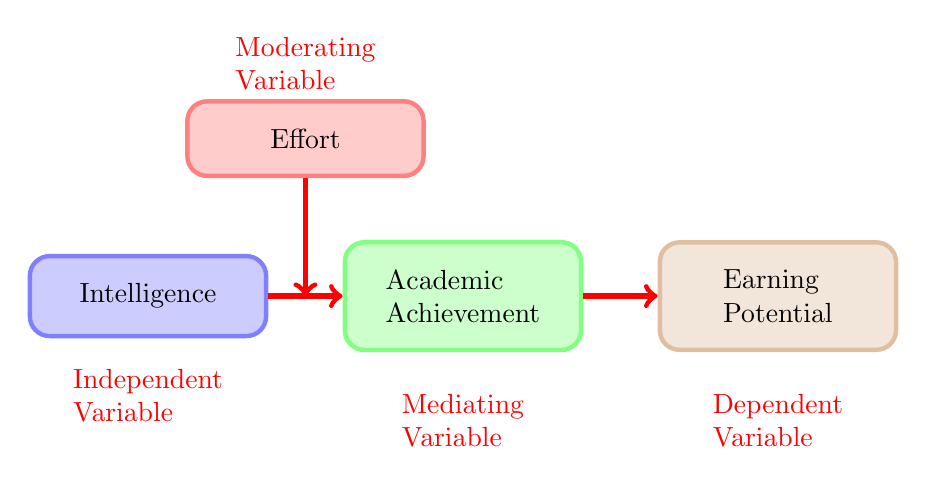
\begin{tikzpicture}
		\node[box01] (box01) [draw, label={[yshift=-2.25cm,align=left]Independent \\ Variable}] at (0,0) {Intelligence};
		\node[box02] (box02) [draw, label={[align=left]Moderating \\ Variable}] at (2,2) {Effort};
		\node[box03] (box03) [draw, label={[yshift=-2.75cm,align=left]Mediating \\ Variable}, align=left] at (4,0) {Academic \\ Achievement};
		\node[box04] (box04) [draw, label={[yshift=-2.75cm,align=left]Dependent \\ Variable}, align=left] at (8,0) {Earning \\ Potential};
		
		% Draw the arrows		
		\draw [->,red,line width=2pt] [out=0]  (box01) 
		to [in=180] (box03);
		\draw [->,red,line width=2pt] [out=0]  (box03) 
		to [in=180] (box04);
		\draw [->,red,line width=2pt] [out=270]  (box02) 
		to [in=90] (2,0);
				
		\end{tikzpicture}
		\caption{Types of Variables}
		\label{02:fig03}
	\end{figure}
\end{center}

In the above illustration, a person's intelligence is an independent variable that influences academic achievement which, in turn, influences earning potential, making academic achievement a mediating variable. Effort independently influences academic achievement along with intelligence so it is considered a moderating variable. To apply measures to this system, if a researcher believes that intelligence influences students' academic achievement, then a measure of intelligence, such as an IQ score, would be the independent variable while a measure of academic success, grade point average, would be the dependent variable. If the effect of intelligence on academic achievement is also dependent on the students' effort then ``effort'' becomes a moderating variable and it could be measured by the number of hours spent studying. Incidentally, it would be reasonable to also view effort as the independent variable and intelligence as a moderating variable. Finally, the dependent variable, earning potential, could be measured by the salary offered to a graduate.

\subsubsection{Attributes of a Good Theory}

Theories are simplified and are often only partial explanations of complex social reality. As such, there can be good explanations or poor explanations, and consequently, there can be good theories or poor theories. How can the ``goodness'' of a theory be evaluated? Different criteria have been proposed by different researchers, the more important of which are listed below:

\begin{itemize}

	\item \Gls{logicalconsistency}: Are the theoretical constructs, propositions, boundary conditions, and assumptions logically consistent with each other? If some of these ``building blocks'' of a theory are inconsistent with each other (\eg, a theory assumes rationality, but some constructs represent non-rational concepts), then the theory is a poor theory.

	\item \Gls{explanatorypower}: How much does a given theory explain (or predict) reality? Good theories obviously explain the target phenomenon better than poor theories, as often measured by the ``variance explained value'' (known as $ R^2 $) in regression equations.

	\item \Gls{falsifiability}: British philosopher Karl Popper stated in the 1940's that for theories to be valid, they must be falsifiable. Falsifiability ensures that the theory is potentially disprovable, if empirical data does not match with theoretical propositions, which allows for their empirical testing by researchers. In other words, theories cannot be theories unless they can be empirically testable. Tautological statements, such as ``a day with high temperatures is a hot day'' are not empirically testable because a hot day is defined (and measured) as a day with high temperatures, and hence, such statements cannot be viewed as a theoretical proposition. Falsifiability requires presence of rival explanations it ensures that the constructs are adequately measurable, and so forth. However, note that saying that a theory is falsifiable is not the same as saying that a theory should be falsified. If a theory is indeed falsified based on empirical evidence, then it was probably a poor theory to begin with!

	\item \Gls{parsimony}: Parsimony examines how much of a phenomenon is explained with how few variables. The concept is attributed to 14th century English logician Father William of Ockham (and is often called ``Ockham's razor'' or ``Occam's razor''), which states that among competing explanations that sufficiently explain the observed evidence, the simplest theory (\ie, one that uses the smallest number of variables or makes the fewest assumptions) is the best. Explanation of a complex social phenomenon can always be increased by adding more and more constructs. However, such approach defeats the purpose of having a theory, which are intended to be ``simplified'' and generalizable explanations of reality. Parsimony relates to the degrees of freedom in a given theory. Parsimonious theories have higher degrees of freedom, which allow them to be more easily generalized to other contexts, settings, and populations.

\end{itemize}

\subsubsection{Approaches to Theorizing}

How do researchers build theories? Steinfeld and Fulk\cite{steinfield1990theory} recommend four approaches. The first approach is to build theories inductively based on observed patterns of events or behaviors. Such approach is often called \gls{groundedtheory} because the theory is grounded in empirical observations. This technique is heavily dependent on the observational and interpretive abilities of the researcher, and the resulting theory may be subjective and not confirmable. Furthermore, observing certain patterns of events will not necessarily make a theory, unless the researcher is able to provide consistent explanations for the observed patterns. 

The second approach to theory building is to conduct a bottom-up conceptual analysis to identify different sets of predictors relevant to the phenomenon of interest using a predefined framework. One such framework may be a simple input-process-output framework, where the researcher may look for different categories of inputs, such as individual, organizational, and/or technological factors potentially related to the phenomenon of interest (the output), and describe the underlying processes that link these factors to the target phenomenon. This is also an inductive approach that relies heavily on the inductive abilities of the researcher, and interpretation may be biased by researcher's prior knowledge of the phenomenon being studied.

The third approach to theorizing is to extend or modify existing theories to explain a new context, such as by extending theories of individual learning to explain organizational learning. While making such an extension, certain concepts, propositions, and/or boundary conditions of the old theory may be retained and others modified to fit the new context. This deductive approach leverages the rich inventory of social science theories developed by prior theoreticians, and is an efficient way of building new theories by building on existing ones.

The fourth approach is to apply existing theories in entirely new contexts by drawing upon the structural similarities between the two contexts. This approach relies on reasoning by analogy, and is probably the most creative way of theorizing using a deductive approach. For instance, Markus\cite{markus1987toward} used analogical similarities between a nuclear explosion and uncontrolled growth of networks or network-based businesses to propose a critical mass theory of network growth. Just as a nuclear explosion requires a critical mass of radioactive material to sustain a nuclear explosion, Markus suggested that a network requires a critical mass of users to sustain its growth, and without such critical mass, users may leave the network, causing an eventual demise of the network.

\section{Propositions, Hypothesis, and Models}

In seeking explanations to an observed phenomenon it is not adequate just to identify key constructs underlying that phenomenon, it is important to also state the patterns of the relationships between constructs. Such patterns of relationships are called propositions. A proposition, thus, is a conjectural relationship between constructs that is stated in a declarative form. An example of a proposition is: ``An increase in student intelligence leads to an increase in academic achievement.'' (This proposition was illustrated in Figure \ref{02:fig03}.) A proposition does not need to be true but it must be testable so its truth can be determined. Propositions are generally derived from either logic (deduction) or observation (induction).

Because propositions are associations between abstract constructs, they cannot be tested directly. Instead, they are tested indirectly by examining the relationship between the corresponding measures (variables) of those constructs. The formulation of a proposition is called a \gls{hypothesis}. Since IQ scores and grade point average are operational measures of intelligence and academic achievement respectively, the proposition stated above can be specified in form of a hypothesis: ``An increase in students' IQ score leads to an increase in their grade point average.'' Propositions are generated from theory while hypotheses are generated from empirical evidence. Hence, hypotheses are testable using observed data and may be rejected if the data do not support them. 

Hypotheses are said to be either strong or weak. ``Students' IQ scores are related to their academic achievement'' is an example of a weak hypothesis since it indicates neither the directionality of the hypothesis (i.e., whether the relationship is positive or negative) nor its causality (i.e., whether intelligence causes academic achievement or academic achievement causes intelligence). A stronger hypothesis is ``students' IQ scores are positively related to their academic achievement,'' which indicates the directionality but not the causality. A still better hypothesis is ``students' IQ scores have positive effects on their academic achievement,'' which specifies both the directionality and the causality (i.e., intelligence causes academic achievement, and not the reverse).

Also note that hypotheses should clearly specify independent and dependent variables. In the hypothesis, ``students' IQ scores have positive effects on their academic achievement,'' it is clear that intelligence is the independent variable (the ``cause'') and academic achievement is the dependent variable (the ``effect''). Further, it is also clear that this hypothesis can be evaluated as either true (if higher intelligence leads to higher academic achievement) or false (if higher intelligence has no effect on or leads to lower academic achievement). Statements such as ``students are generally intelligent'' or ``all students can achieve academic success'' are not hypotheses because they do not specify independent and dependent variables nor do they specify a directional relationship that can be evaluated as true or false.

\subsection{Theories and Models}

A term often used in conjunction with theory is \gls{model}. A model is a representation of all or part of a system that is constructed to study that system (e.g., how the system works or what triggers the system). While a theory tries to explain a phenomenon, a model tries to represent a phenomenon in an understandable way. Models are often used to make important decisions that are based on a given set of inputs. For instance, marketing managers may use models to decide how much money to spend on advertising for different product lines based on parameters such as prior year's advertising expenses, sales, market growth, and competing products. Likewise, weather forecasters use models to predict future weather patterns based on parameters such as wind speeds, air pressure, temperature, and humidity. While these models are useful, they do not explain the theory behind advertising budgets or weather forecasting. 

Models may be of different kinds, such as mathematical models, network models, and path models. Models can also be descriptive, predictive, or normative. Descriptive models are frequently used for representing complex systems, for visualizing variables and relationships in such systems. Predictive models (e.g., a regression model) allow forecast of future events. Normative models are used to guide activities along commonly accepted norms or practices. Models may also be static if it represents the state of a system at one point in time or dynamic if it represents a system's evolution over time.

The process of theory or model development may involve both inductive and deductive reasoning, as described in Chapter 1, as shown in the following figure. Induction occurs when we observe a fact and ask, ``Why is this happening?'' while deduction occurs when we have a theory and ask, ``Is this supported by observable facts?'' Both induction and deduction leads to preliminary conclusions that are then tested in order to develop a final model of the phenomenon. Researchers must be able to move back and forth between inductive and deductive reasoning if they are to post extensions or modifications to a given model or theory, or built better ones, which are the essence of scientific research. This process is illustrated in Figure \ref{02:fig04}.

\begin{center}
	\begin{figure}[H]
		\tikzstyle{box01}=[rectangle,draw=blue!50,fill=blue!20,ultra thick,
		inner sep=10pt,minimum width=3cm,rounded corners=.25cm]
		\tikzstyle{box02}=[rectangle,draw=red!50,fill=red!20,ultra thick,
		inner sep=10pt,minimum width=3cm,rounded corners=.25cm]
		\tikzstyle{box03}=[rectangle,draw=green!50,fill=green!20,ultra thick,
		inner sep=10pt,minimum width=3cm,rounded corners=.25cm]
		\tikzstyle{box04}=[rectangle,draw=brown!50,fill=brown!20,ultra thick,
		inner sep=10pt,minimum width=3cm,rounded corners=.25cm]
		%		\tikzstyle{every label}=[red]
		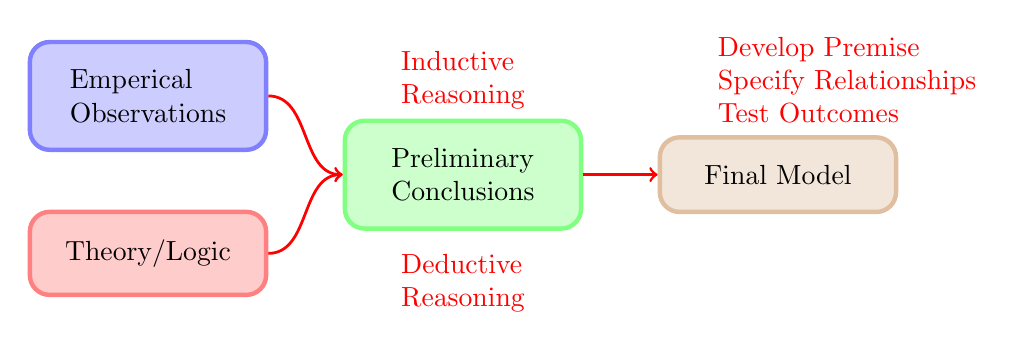
\begin{tikzpicture}
		\node[box01] (box01) [draw, align=left] at (0,2) {Emperical \\ Observations};
		\node[box02] (box02) [draw, align=left] at (0,0) {Theory/Logic};
		\node[box03] (box03) [draw, align=left] at (4,1) {Preliminary \\ Conclusions};
		\node[box04] (box04) [draw, align=left] at (8,1) {Final Model};
		
		% Draw the arrows		
		\draw [->,red,line width=1pt] [out=0]  (box01) 
		to [in=180] (box03) node[above, align=left, yshift=20] {Inductive \\ Reasoning};
		\draw [->,red,line width=1pt] [out=0]  (box02) 
		to [in=180] (box03) node[below, align=left, yshift=-25] {Deductive \\ Reasoning};
		\draw [->,red,line width=1pt] [out=0]  (box03) 
		to [in=180] (box04) node[above, align=left, yshift=15, xshift=25] {Develop Premise \\ Specify Relationships \\ Test Outcomes};
		
		\end{tikzpicture}
		\caption{The Model-Building Process}
		\label{02:fig04}
	\end{figure}
\end{center}

\section{Inductive or Deductive Approaches}

Theories are used to structure research at the same time that the research structures theory. The reciprocal relationship between theory and research becomes more evident to researchers as they determine whether an inductive or deductive approach is best. Often, researchers find that a single approach is not ideal and projects iterate over many cycles of inductive/deductive approaches. It is common for a researcher to start with an \gls{inductiveresearch} approach and postulate a new theory then switch to a \gls{deductiveresearch} approach to test that theory. Later the researcher may return to an inductive approach to expand and refine the theory, followed by another round of deductive methods to test the new theory.

\subsection{Inductive Research}

\marginpar{Saying that inductive research leads to a ``theory'' may be a bit of a stretch. More accurately, it leads to empirical generalizations.}In inductive research, a researcher begins by collecting data that are relevant to the topic of interest. Once a substantial amount of data have been collected, the researcher will start to look for trends or correlations and then develop the theory that explains those patterns. Thus, an inductive approach moves from data to theory, or from specific instances to general explanations and is often referred to as a ``bottom-up'' approach. Figure \ref{02:fig05} broadly outlines the process used with an inductive approach to research.

\begin{center}
	\begin{figure}[H]
		\tikzstyle{box1}=[rectangle,draw=cyan!90,fill=cyan!10,ultra thick,
		inner sep=10pt,minimum width=3.5cm,minimum height=1.5cm,
		rounded corners=.25cm]
		\tikzstyle{box2}=[rectangle,draw=cyan!90,fill=cyan!25,ultra thick,
		inner sep=10pt,minimum width=3.5cm,minimum height=1.5cm,
		rounded corners=.25cm]
		\tikzstyle{box3}=[rectangle,draw=cyan!90,fill=cyan!40,ultra thick,
		inner sep=10pt,minimum width=3.5cm,minimum height=1.5cm,
		rounded corners=.25cm]
		\tikzstyle{box4}=[rectangle,draw=cyan!90,fill=cyan!55,ultra thick,
		inner sep=10pt,minimum width=3.5cm,minimum height=1.5cm,
		rounded corners=.25cm]			
		\tikzstyle{every label}=[red]
		\begin{tikzpicture}
		\node[box1] (obs)                      {Observations};
		\node[box2] (pat) [above=0.5cm of obs,xshift=2.5cm] {Patterns};
		\node[box3] (hyp) [above=0.5cm of pat,xshift=2.5cm]	{Hypothesis};
		\node[box4] (the) [above=0.5cm of hyp,xshift=2.5cm] {Theory};
				
		% Draw the arrows		
		\draw [->,blue,line width=3pt] [out=0] (obs) to [in=270] (pat);
		\draw [->,blue,line width=3pt] [out=0] (pat) to [in=270] (hyp);
		\draw [->,blue,line width=3pt] [out=0] (hyp) to [in=270] (the);
		
		\end{tikzpicture}
		\caption{Inductive Reasoning}
		\label{02:fig05}
	\end{figure}
\end{center}

Inductive methods are commonly applied to qualitative research projects and are frequently criticized for being too subjective. The goal is, generally, to attempt to understand the dynamics of business practices and use that understanding to draw general conclusions that may apply to other businesses. The result of many qualitative research projects is what is called \gls{groundedtheory}\footnote{Grounded theory was first discussed by Glaser and Strauss in the late $ 1960 $'s but has been discussed in many journal articles and books. See, for example, Strauss, Anselm, and Juliet Corbin\cite{strauss1994grounded}.} where the researcher starts with no preconceived notions and generates a new theory from the data analysis.

Following are three examples of inductive methods research.

\begin{itemize}
	\item Bansal, Pratima, and Roth\cite{bansal2000companies} conducted a study concerning why corporations ``go green.'' They collected data from 53 firms in the United Kingdom and Japan and analyzed that data to formulate a theory.

	\item Sharma\cite{sharma2000managerial} sent surveys to $ 3-5 $ senior managers of $ 110 $ Canadian oil and gas companies with annual sales in excess of $ \$20 $ million. The surveys were analyzed and the researcher concluded that managers of these companies must be influenced to embrace environmental issues as a corporate goal, but that must be done within the context of the corporate structure.  

	\item Sia and Gopa\cite{sia2009employees} used an inductive method to analyze effect on diversity of the ``psychological contract'' between a corporation and its employees. A psychological contract is described as what the employee ``...believes he or she has agreed to...'' rather than what is actually in the employment contract. They administered two different surveys to $ 207 $ managers of public sector units in Orrisa, India. They found that certain minority groups tended to ``...protect each other when required, particularly during the time of crisis.'' However, members of the dominant group did not engage in that type of behavior, leading to ``...a feeling of non-inclusiveness.''

\end{itemize}

In addition to the research studies discussed above, several papers have been published by various journals encouraging inductive research methods, especially in analyzing case studies. For example, Eisenhardt and Graebner\cite{eisenhardt2007theory} published an article in the \textit{Academy of Management Journal} that suggested  a process for generating theory from multiple case studies and encouraged management researchers to consider the role of theory-generation in their case studies. 

\subsection{Deductive Research}

In deductive research, a researcher begins with a theory of interest and then collects data to test that theory. Thus, a deductive approach moves from a general explanation of some phenomenon to specific instances that prove, or disprove, the phenomenon and is often referred to as a ``top-down'' approach. Figure \ref{02:fig06} broadly outlines the process used with a deductive approach to research.

\begin{center}
	\begin{figure}[H]
		\tikzstyle{box1}=[rectangle,draw=purple!90,fill=purple!10,ultra thick,
		inner sep=10pt,minimum width=3.5cm,minimum height=1.5cm,
		rounded corners=.25cm]
		\tikzstyle{box2}=[rectangle,draw=purple!90,fill=purple!25,ultra thick,
		inner sep=10pt,minimum width=3.5cm,minimum height=1.5cm,
		rounded corners=.25cm]
		\tikzstyle{box3}=[rectangle,draw=purple!90,fill=purple!40,ultra thick,
		inner sep=10pt,minimum width=3.5cm,minimum height=1.5cm,
		rounded corners=.25cm]
		\tikzstyle{box4}=[rectangle,draw=purple!90,fill=purple!55,ultra thick,
		inner sep=10pt,minimum width=3.5cm,minimum height=1.5cm,
		rounded corners=.25cm]			
		\tikzstyle{every label}=[red]
		\begin{tikzpicture}
		\node[box1] (the)                                   {Theory};
		\node[box2] (hyp) [below=0.5cm of the,xshift=2.5cm] {Hypothesis};
		\node[box3] (obs) [below=0.5cm of hyp,xshift=2.5cm] {Observations};
		\node[box4] (con) [below=0.5cm of obs,xshift=2.5cm] {Confirmation};
				
		% Draw the arrows		
		\draw [->,violet,line width=3pt] [out=270] (the) to [in=180] (hyp);
		\draw [->,violet,line width=3pt] [out=270] (hyp) to [in=180] (obs);
		\draw [->,violet,line width=3pt] [out=270] (obs) to [in=180] (con);
		
		\end{tikzpicture}
		\caption{Deductive Reasoning}
		\label{02:fig06}
	\end{figure}
\end{center}

Deductive methods are commonly applied to quantitative research projects and are often considered the ``gold standard'' of methods, especially among researchers in the natural sciences. The goal is, generally, to test existing theories to see if they are valid in cases that have not been previously considered. Following are a few example studies that use a deductive approach.

\begin{itemize}
	\item Parboteeah, Paik, and Cullen\cite{parboteeah2009religious} studied the influence of religion on the workplace. They used data from more then $ 44 $ thousand individuals in $ 39 $ countries to determine if Buddhism, Christianity, Hindusim, and Islam influenced both extrinsic and intrinsic work values. They found that the results ``...generally support the posited hypotheses, confirming that religion is positively related to work values.'' Because the study began with hypotheses and tested those hypotheses against gathered data this is a deductive methodology.

	\item Hackman and Oldham\cite{hackman1976motivation} used existing theory to develop a model to predict the conditions that will motivate employees to perform effectively on their jobs. They tested $ 658 $ employees who worked at $ 62 $ different jobs in seven organizations and found that the results support the validity of their model.

	\item Delaney and Huselid\cite{delaney1996impact} investigated the relationship between human resource management and perceptions of organizational performance. They came up with two hypotheses and then gathered data to test those hypotheses. The result of their study is that positive human resources practices (like training programs) have a positive correlation with the perception of the organizational performance. 
\end{itemize}

\subsection{Complementary Approaches}

While inductive and deductive approaches to research seem quite different, they are complementary in the sense that one approach creates theories and the other tests theories. In some cases, researchers plan for their research to include multiple phases, one inductive and the other deductive. In other cases, a researcher might begin a study with the plan to only conduct either inductive or deductive research but then discover that the other approach is needed to develop a full picture.

One such example is a research project completed by Lawrence Sherman and Richard Berk\cite{sherman1984specific}. They conducted an experiment to test two competing theories of the effects of punishment on deterring domestic violence. Specifically, Sherman and Berk hypothesized that deterrence theory would provide a better explanation of the effects of arresting accused batterers than labeling theory. Deterrence theory predicts that arresting an accused spouse batterer will reduce future incidents of violence while labeling theory predicts that arresting accused spouse batterers will increase future incidents. 

Sherman and Berk found, after conducting an experiment with the help of local police in one city, that arrest did in fact deter future incidents of violence, thus supporting their hypothesis that deterrence theory would better predict the effect of arrest. After conducting this research, they and other researchers went on to conduct similar experiments in six additional cities but the results from these follow-up studies were mixed. In some cases, arrest deterred future incidents of violence but in other cases, it did not. This left the researchers with new data that they needed to explain. The researchers next took an inductive approach in an effort to make sense of their latest empirical observations. The new studies revealed that arrest seemed to have a deterrent effect for those who were married and employed but that it led to increased offenses for those who were unmarried and unemployed. In the end, the researchers turned to control theory and predicted that having some stake in conformity through the social ties provided by marriage and employment would deter future violence. This research project is a good example of one that evolves through several iterations of induction/deduction.

\section{Summary}

\begin{center}
	\begin{tkawybox}{Summary}
		\begin{itemize}
			\setlength{\itemsep}{0pt}
			\setlength{\parskip}{0pt}
			\setlength{\parsep}{0pt}
			
			\item A paradigm is the researcher's own frames of reference, or believe systems. Researchers should be aware of their own paradigms and take steps to ensure that it will not introduce bias into the research project.
			\item Theories are explanations of a natural or social behavior, event, or phenomenon. It is a system of constructs, or concepts, and propositions that describe the relationships between those constructs. Theories are built by defining the constructs being evaluated and then determining the propositions that link the constructs.
			\item A proposition is the relationship between constructs. A proposition does not need to be true but it must be testable so its truth can be determined. The formulation of a proposition is called a hypothesis. A model is a representation of all or part of a system that is constructed to study that system. 
			\item Inductive research begins with observations and attempts to build a theory from those observations. Deductive research begins with a theory and tests observations to determine if the theory is valid.
		\end{itemize}
	\end{tkawybox}
\end{center}

